\documentclass[11pt]{article}
\usepackage[margin=1.05in]{geometry}
\usepackage{graphicx}
\usepackage{booktabs}
\usepackage{amsmath}
\usepackage{array}
\usepackage{float}
\usepackage{placeins}
\usepackage[hidelinks]{hyperref}
\usepackage[round]{natbib}
\usepackage{microtype}

\title{What Gives You Away?\\ \Large How Linguistic Cues Move User Readouts Across Three Language Models}
\author{Cat McGee}
\date{August 2026}

\begin{document}
\maketitle

\begin{abstract}
Small differences in wording may alter the demographic signals encoded in a
language model's representation of a user. We test this possibility by placing
controlled linguistic edits inside otherwise identical conversations. The
main experiment compares 1,025 pairs built from 100 base messages in Llama 3.2
3B. A shared set of 505 pairs is also tested in Llama 3.1 8B and OLMo 2 32B.
Simple classifiers act as measuring tools: they show how much each change moves
internal signals related to the user's age, gender, education, or socioeconomic
status.

In the main experiment, 30 of the 36 combinations of writing cue and user
attribute produce a statistically reliable shift after accounting for the
number of tests; 28 move more than a matched synonym edit. The age readout is
especially sensitive to personal context, emoji, and slang. The education
readout is most affected by grammar and personal context, while the
socioeconomic readout is most affected by price language and personal context.
The gender pattern is less consistent. The broad ordering appears again in both
larger models and under different conversation wording. Some style effects
fade after later messages, but the effect of personal context lasts longer.

These results show that small differences in wording can change the demographic
signals measured inside a model. They do not show that those signals are
correct, that the model has identified a person's real attributes, or that it
uses this information when writing its response.
\end{abstract}

\section{Introduction}

Writing has long been known to carry information about its author
\citep{stamatatos2009survey,schler2006blogs}. In a dialogue system, a related
question is whether a controlled change to one user turn alters a demographic
probe output while the rest of the conversation remains unchanged. This
isolates sensitivity to a linguistic cue from demographic prediction over an
uncontrolled corpus.

This study uses the age, gender, education, and socioeconomic readouts from
TalkTuner \citep{chen2024dashboard}. A linear probe converts a hidden state into
class logits, providing a fixed instrument for measuring how an edit changes
the representation. A separate five-seed probe ensemble is fitted for each of
three models. Rows sharing a source generator and numeric index remain
together during training and evaluation, so related source rows cannot cross
partitions.

The probes were trained on full conversations, so every primary measurement is
also made in a full conversation. Two independently worded neutral preludes
place the edited message at the current user turn. Two further conditions move
that message one or two user turns into the past. The paired conversations
always share the same assistant messages, preventing a generated response from
becoming an uncontrolled mediator.

The experiment maps nine cue categories to four readouts, evaluates that map
in three checkpoints, and measures selected effects again after one and two
later user turns. It also varies the neutral prelude, the readout phrase, and
the probe split seed. Cue order is similar across models, with greater
variation in lower-ranked cues and temporal persistence.

\section{Related work}

\paragraph{User representations.}
TalkTuner trains linear probes for a conversational user's age, gender,
education, and socioeconomic status, then exposes those estimates in an
interactive dashboard \citep{chen2024dashboard}. Related work examines implicit
personalization and stereotype-driven user representations
\citep{neplenbroek2025implicit}. This study measures the sensitivity of those
readouts to controlled input edits.

\paragraph{Probing and interpretation.}
The probing literature distinguishes decodable information from information a
model uses in its own predictions \citep{hewitt2019probes,voita2020mdl,
elazar2021amnesic}. Our paired contrast identifies the effect of a particular
text edit on a fixed probe output in a constructed conversation. It says
nothing by itself about label truth or downstream generation.

Prompt sensitivity is a related measurement problem: small changes to an
evaluation prompt can alter model scores without changing the underlying task
\citep{hua2025prompt}. Sensitivity to readout phrasing is evaluated by repeating
the cue matrix under three paraphrases of each attribute's readout phrase.

\paragraph{Style and demographic inference.}
Stylometric systems use vocabulary, syntax, spelling, and punctuation to infer
properties of authors and documents \citep{stamatatos2009survey}. Such
correlations can reflect population structure, topic, sampling choices, and
stereotypes. A paired design isolates changes in probe output while the request
and conversation are held fixed.

\section{Method}
\label{sec:method}

\subsection{Model and readouts}

The main experiment uses Llama 3.2 3B Instruct \citep{meta2024llama32}. We
repeat the study on Llama 3.1 8B Instruct, a larger checkpoint from the same
model family, and OLMo 2 32B Instruct, a larger independently developed model
\citep{grattafiori2024llama,olmo2024furious}.
{\small\raggedright
The exact checkpoint identifiers are \path{unsloth/Llama-3.2-3B-Instruct},
\path{unsloth/Meta-Llama-3.1-8B-Instruct}, and
\path{allenai/OLMo-2-0325-32B-Instruct}.\par}
Their immutable revisions are recorded in the public release described below.
This is a cross-model comparison, not a factorial test of parameter count:
model size, family, and training recipe are not independently varied.

Each conversation is formatted with the relevant model's chat template. At
the start of a new assistant turn, we append an attribute-specific phrase such
as ``I think the education level of this user is''. A multinomial logistic
regression reads the hidden state at the final token of that phrase. For hidden
state $h$,

\[
  p(y=c\mid h)=\operatorname{softmax}_c(Wh+b).
\]

The four readouts are age, gender, education, and socioeconomic status. We fit
the probes separately in each model using the same complete TalkTuner
conversations and recipe. For each attribute, 300 label-complete sets sharing
a generator folder and numeric source index are sampled. Each set stays within
one 70/15/15 train, layer-selection, or test partition. The middle split
selects the layer; the final split is used only for reporting. We fit five
split seeds. Table~\ref{tab:probe-accuracy} reports held-out balanced accuracy.
Every attribute and seed exceeds the pre-specified .75 gate.

\begin{table}[H]
\centering
\small
\begin{tabular}{lrrr}
\toprule
Readout & Llama 3.2 3B & Llama 3.1 8B & OLMo 2 32B \\
\midrule
Age & .963 & .958 & .972 \\
Gender & .929 & .949 & .889 \\
Education & .957 & .957 & .966 \\
Socioeconomic status & .975 & .970 & .978 \\
\bottomrule
\end{tabular}
\caption{Mean held-out balanced accuracy across five independently split probe
seeds. The lowest individual score is .822 for the 32B gender readout.}
\label{tab:probe-accuracy}
\end{table}

For a matched edit from conversation $A$ to conversation $B$, the class-logit
change is

\[
  \Delta z_c=w_c^{\top}(h_B-h_A).
\]

The intercept cancels. Both variants use the same model, conversation shell,
readout phrase, probe seed, and readout position. The outcome for one probe is
$\max_c|\Delta z_c|$. This measures how far the edit moves the attribute
readout without privileging a class direction. Consequently, the metric does
not identify whether an age readout shifted toward an older or younger class.
Each attribute and model has a separately fitted probe, so raw logit units are
comparable only among cues evaluated with the same readout and model.
Cross-model analyses use within-readout cue ranks, signs relative to control,
corrected significance, and dimensionless retention ratios.

\subsection{Controlled pairs}

The dataset contains 1,025 pairs over 100 user messages about travel, cooking,
small talk, technical support, health, finance and shopping, and work or
study. Every base has a neutral synonym control; the number of cue edits varies
by category. Table~\ref{tab:data} summarizes the complete dataset.

\begin{table}[H]
\centering
\small
\begin{tabular}{lr@{\qquad}lr}
\toprule
Category & Pairs & Category & Pairs \\
\midrule
Orthography & 184 & Personal context & 111 \\
Emoji & 100 & Grammatical complexity & 100 \\
Random-synonym control & 100 & Contraction/formality & 94 \\
Slang & 94 & Affect language & 82 \\
US-to-UK spelling & 82 & Price language & 78 \\
\bottomrule
\end{tabular}
\caption{Released controlled pairs. Orthography
includes lowercasing, punctuation removal, and typographical errors. Random
synonym replacements provide a matched lexical-movement floor.}
\label{tab:data}
\end{table}

Personal-context edits add either direct personal information, such as an age
or education statement, or an indirect contextual marker, such as retirement
or a family reference. The category therefore does not imply that the target
attribute is always stated directly. Price edits make low-cost or high-cost
preferences explicit, through lexical replacement or an added qualifier.
Emoji edits append one symbol. Grammar edits rewrite one sentence with more
complex syntax while preserving the request. Orthographic edits alter
capitalization, punctuation, or spelling. Pairs were reviewed for naturalness,
a clear target manipulation, and preservation of the underlying request. The
dataset is a set of controlled contrasts rather than a representative sample
of human writing.

Every base also has a neutral synonym replacement. For each cue category, the
analysis compares its movement with the control movement for the same base
message. This subtracts the background movement produced by changing a word at
all.

\subsection{Conversation construction}

Every pair is rendered in four conversation views. Two primary views place the
target after independently worded neutral preludes:

\begin{quote}
\small
\textbf{User:} I could use your help with a question.\\
\textbf{Assistant:} Of course. What would you like help with?\\
\textbf{User:} [target message]
\end{quote}

The second shell uses different but semantically similar wording. The other two
views place one or two fixed assistant--user exchanges after the target before
the readout is taken. In every view, the two variants have the same number and
order of messages and differ at exactly one user turn. The full 3B release
contains 4,100 rendered conversation rows.

The default readout phrase is used in all four views. Three paraphrases are
also evaluated on one current-turn shell, yielding 7,175 pair-by-condition
measurements at 3B. The paraphrases vary wording while preserving the requested
attribute. Evaluated forms include ``Based on this conversation, this user's
age group is'' and ``My estimate of the user's age is''. A fixed panel of 505
pairs over 48 bases is evaluated in all three models, keeping the cross-model
comparison exactly matched. The panel contains every pair associated with the
first 48 base identifiers in the canonical order of the released dataset. It
was fixed in the study plan before the 8B and 32B cue-map runs. Selection was
deterministic rather than random or stratified; no larger-model result was used
to choose a base. As a descriptive coverage check, the panel's 3B cue ranks
correlate $.917$ with the full 3B ranks after ranking within readout; the four
readout-specific correlations range from $.833$ to $.983$.

\subsection{Estimands and inference}

For each pair and readout, movement is averaged across five probe seeds. The
primary estimate then averages the two current-turn conversation shells. For
cue category $k$ and base message $i$, let $M_{ik}$ be that average and
$M_{i0}$ the corresponding random-synonym control. The reported effect is

\[
  \hat{\tau}_k=\frac{1}{|I_k|}\sum_{i\in I_k}(M_{ik}-M_{i0}).
\]

The base message is the independent unit. Confidence intervals use 5,000
base-cluster bootstrap draws. Two-sided $p$-values use 10,000 sign flips at the
base level. Benjamini--Hochberg correction covers the 36 non-control
cue-by-attribute cells. Probe seeds and conversation shells are repeated
measurements and are not counted as independent observations.

For temporal persistence, we divide the later-turn paired effect by the
current-turn paired effect. The ratio is computed as a ratio of means, with a
base-cluster bootstrap interval. Conversation-shell and readout-phrase
robustness are summarized by ranking the nine cues separately within each
readout, then pooling the 36 ranks for a Spearman correlation. This avoids
comparing arbitrary scales from different probes.

Each larger model is compared with the 3B panel by (i) pooled and per-readout
correlations of within-readout cue ranks, (ii) sign and corrected-significance
agreement for the 30 3B-significant cells, and (iii) rank and absolute
agreement for six selected retention cells. We do not attach a
cell-independence $p$-value to the cross-model rank correlation because cells
sharing cues and readouts are structured, not independent observations.

\subsection{Departure from the planned cross-model endpoints}

The fixed plan named a Spearman correlation over the 36 raw cue-by-readout
effects and agreement on the highest-moving readout for each cue. During
analysis, we found that both endpoints compare logits from independently fitted
probes with arbitrary scales. We therefore replaced them with cue ranks
computed separately within each readout and then pooled those 36 ranks. This is
a post-plan change to the cross-model analysis. The cell-level estimates,
inference, signs, corrected-significance comparisons, and retention endpoints
are unchanged; no raw magnitude comparison across probes is interpreted.

\section{Results}
\label{sec:results}

\subsection{The 3B cue map}

Figure~\ref{fig:matrix} gives the complete 1,025-pair 3B cue map. Thirty of 36
cells have $q<.05$: 28 move more than their matched synonym controls and two
move less. The two negative cells are contraction-expansion-to-education and
US-to-UK-spelling-to-socioeconomic-status. Both belong to cue categories whose
overall movement is small.

\begin{figure}[H]
\centering
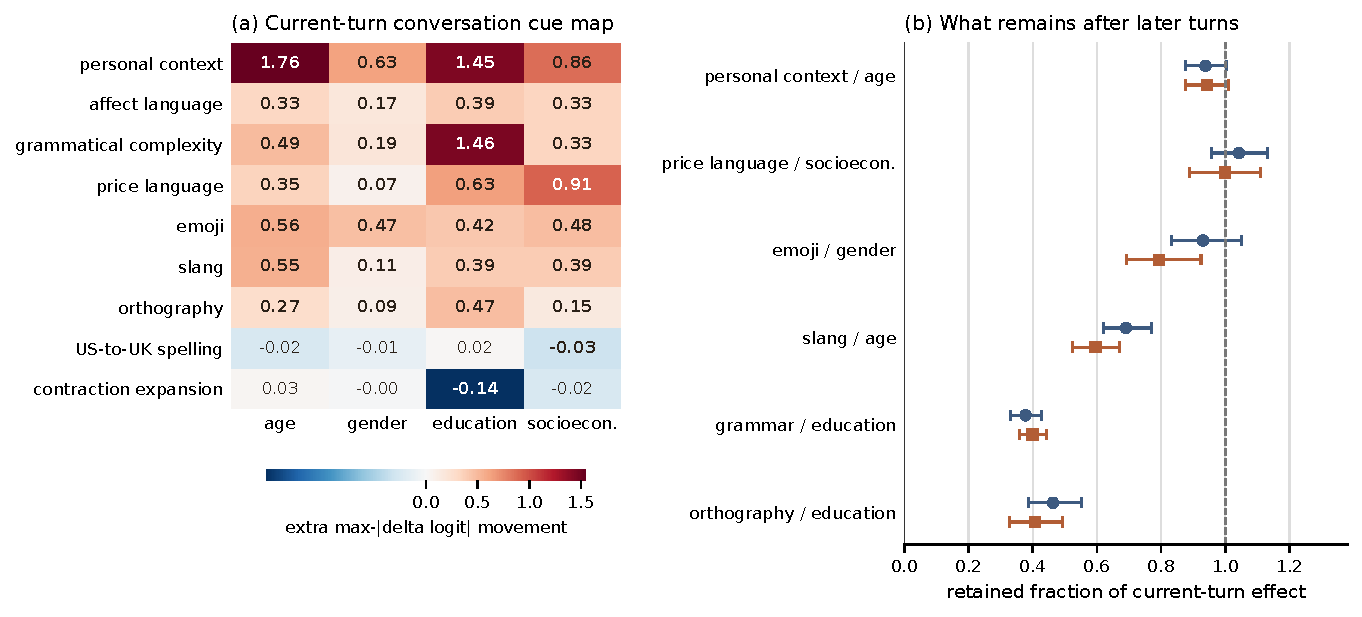
\includegraphics[width=\linewidth]{fig_conversation_sensitivity.pdf}
\caption{The 1,025-pair 3B experiment. (a) Movement relative to the
matched random-edit floor, averaged across two current-turn shells and five
full-conversation probe seeds. Bold cells have $q<.05$ after correction over
36 comparisons. (b) Fraction of selected current-turn effects retained after
one or two later user turns; bars are base-bootstrap 95\% intervals.}
\label{fig:matrix}
\end{figure}

\begin{table}[H]
\centering
\small
\begin{tabular}{llrr}
\toprule
Cue & Readout & Extra movement & 95\% CI \\
\midrule
Personal context & age & 1.756 & [1.517, 2.003] \\
Emoji & age & 0.565 & [0.479, 0.655] \\
Personal context & gender & 0.625 & [0.492, 0.767] \\
Emoji & gender & 0.466 & [0.348, 0.600] \\
Grammatical complexity & education & 1.458 & [1.233, 1.680] \\
Personal context & education & 1.448 & [1.185, 1.726] \\
Price language & socioeconomic status & 0.915 & [0.774, 1.053] \\
Personal context & socioeconomic status & 0.860 & [0.721, 1.005] \\
\bottomrule
\end{tabular}
\caption{The two largest numerical effects within each readout in the full 3B
experiment. Extra movement is category movement minus matched synonym-control
movement, measured in maximum absolute class-logit change. Values should be
compared within a readout, not between separately fitted probes.}
\label{tab:cues}
\end{table}

Within-readout rankings differ by attribute. Personal context leads age,
followed by emoji and slang. Personal context and emoji lead gender. Grammar
and personal context are nearly tied at the top of education. Price and
personal context lead socioeconomic status. Price is also third for education,
and grammar is fourth for age,
demonstrating that the matrix is not a one-cue, one-readout assignment.

Contraction expansion and US-to-UK spelling do not show a corrected positive
effect. Contraction expansion reduces education movement by 0.136, and
US-to-UK spelling reduces socioeconomic movement by 0.028; the other six cells
do not survive correction. Thus, an observable style change need not produce a
positive corrected effect.

Categorical flip rates provide a secondary effect-size summary but depend on
the starting margin. Grammatical complexity changes the ensemble education
label in 27\% of its pairs, price language changes the ensemble socioeconomic
label in 37\%, emoji changes the ensemble gender label in 30\%, and slang
changes the ensemble age label in 22\%.

\subsection{Cross-model agreement}

The cue map has strong cross-model agreement (Figure~\ref{fig:cross}).
On the shared panel, the pooled within-readout cue-rank correlation is
$\rho=.938$ for 8B against 3B and $\rho=.850$ for 32B against 3B. All 30 cells that are
corrected-significant at 3B retain a positive above-control effect in both
models. Twenty-nine of those 30 remain corrected-significant in each larger
model. The non-significant 8B cell is contraction-expansion-to-gender; the
non-significant 32B cell is US-to-UK-spelling-to-education. Across all 36 cells,
32 are corrected-significant at 8B and 33 at 32B.

\begin{figure}[H]
\centering
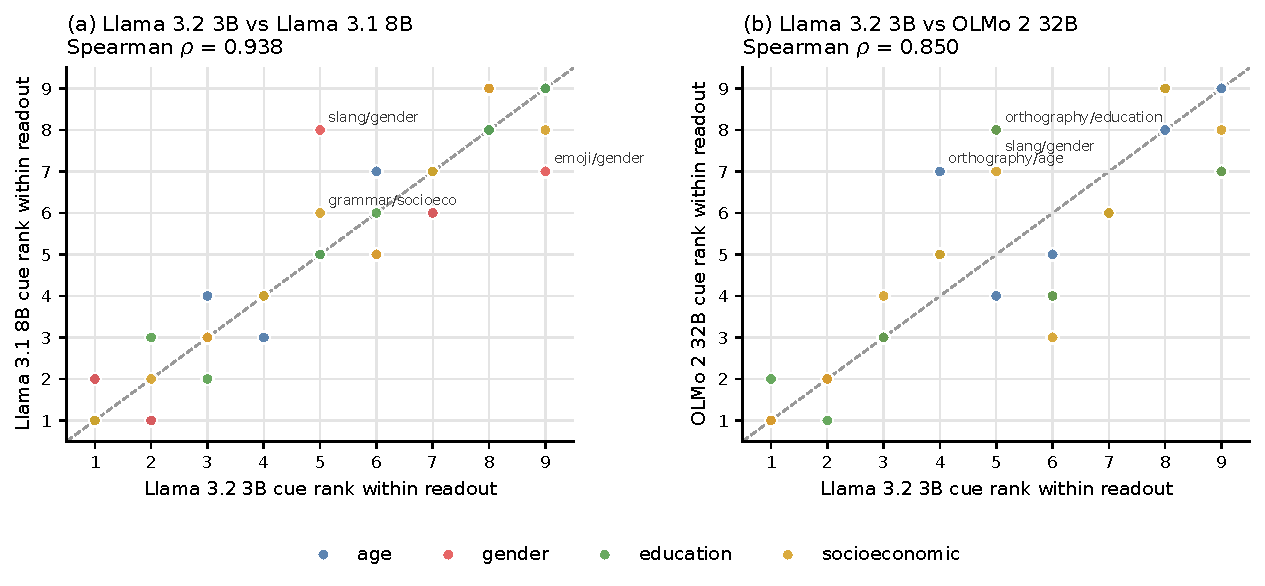
\includegraphics[width=\linewidth]{fig_cross_model.pdf}
\caption{Cross-model agreement on the shared 505-pair, 36-cell cue map. The
nine cues are ranked separately within each readout; the plotted correlations
pool those ranks. The dashed line marks identical ranks. Labels identify the
three largest rank changes in each comparison.}
\label{fig:cross}
\end{figure}

\begin{table}[H]
\centering
\small
\begin{tabular}{lrrrr}
\toprule
Model & Pooled $\rho$ & Readout $\rho$ range & Same sign & Still $q<.05$ \\
\midrule
Llama 3.1 8B & .938 & .850--.983 & 30/30 & 29/30 \\
OLMo 2 32B & .850 & .817--.900 & 30/30 & 29/30 \\
\bottomrule
\end{tabular}
\caption{Cross-model endpoints relative to the shared-panel 3B map. Cue ranks
are computed within each readout before pooling. Sign and
corrected-significance columns cover the 30 3B-significant cells.}
\label{tab:crossmodel}
\end{table}

Agreement is also present in the readout-specific rankings. Personal context
and slang rank first and second for age in all three models. Price and personal context
occupy the top two socioeconomic positions, with their order reversed in the
3B panel. Grammar and personal context are the top two education cues in both
Llama models; OLMo places personal context, orthography, and grammar in its top three.
Gender is less stable. Emoji ranks first for the 3B gender readout but third at
8B and 32B, behind personal context and slang. These rankings concern cue order
within a readout and do not support magnitude comparisons between demographic
readouts.

\subsection{Stability across context and readout wording}

The two neutral conversation shells produce similar within-readout cue orders
in every model: pooled $\rho=.971$ in the full 3B analysis, $.967$ at 8B, and
$.992$ at 32B. Cue order is therefore robust to prelude wording.

Variation is larger across readout phrases. Three paraphrases correlate
$.892$--$.929$ with the default phrase in the full 3B run, $.883$--$.933$ at
8B, and $.875$--$.921$ at 32B. Cue order remains similar, but an individual
logit magnitude should not be treated as phrase-invariant.

Probe-seed variation is also substantial. In the full 3B run,
grammar-to-education is positive in all five seeds but ranges from 0.447 to
2.474; emoji-to-age ranges from 0.404 to 0.854. These are separately fitted
instruments, so the analysis averages them rather than treating any one
probe's scale as definitive.

\subsection{Temporal persistence}

The selected cue--readout cells have different time courses.
Table~\ref{tab:persistence} reports the fraction of each current-turn
effect retained after later neutral exchanges in all three models.

Personal context / age retains .90--.98 of its current-turn movement after two
turns in every model. Slang / age falls to .47--.57, and orthography /
education falls to .23--.42. Price / socioeconomic status is nearly unchanged
at 3B and 8B but retains .69 at 32B. Grammar / education also
decays less at 32B than in either Llama model. Across the six selected
cells, the 3B retention ordering correlates $.886$ and $.829$ with 8B after one
and two turns, and $.771$ at both lags with 32B. Personal context is consistently
durable and several style effects attenuate, but the price and emoji results do
not support a uniform content-versus-style distinction in temporal
persistence. The full 3B estimates are similar: after two turns, the six rows
in Table~\ref{tab:persistence} retain .94, 1.00, .79, .60, .40, and .41,
respectively.

\begin{table}[H]
\centering
\small
\begin{tabular}{lrrr}
\toprule
Cue / readout & 3B & 8B & 32B \\
\midrule
\multicolumn{4}{l}{\textit{One turn later}} \\
Personal context / age & 1.01 & 1.04 & 0.95 \\
Price / socioeconomic status & 1.03 & 1.17 & 0.71 \\
Emoji / gender & 0.97 & 1.10 & 0.93 \\
Slang / age & 0.68 & 0.51 & 0.66 \\
Grammar / education & 0.41 & 0.48 & 0.64 \\
Orthography / education & 0.52 & 0.44 & 0.24 \\
\addlinespace
\multicolumn{4}{l}{\textit{Two turns later}} \\
Personal context / age & 0.98 & 0.98 & 0.90 \\
Price / socioeconomic status & 1.01 & 1.15 & 0.69 \\
Emoji / gender & 0.79 & 1.45 & 0.76 \\
Slang / age & 0.57 & 0.47 & 0.51 \\
Grammar / education & 0.43 & 0.46 & 0.66 \\
Orthography / education & 0.41 & 0.42 & 0.23 \\
\bottomrule
\end{tabular}
\caption{Ratio of later-turn to current-turn paired effects on the shared
505-pair panel. Values above one indicate greater measured movement at
the later readout, not a calibrated gain in memory. Bootstrap intervals for
every cell are released with the results.}
\label{tab:persistence}
\end{table}

\section{Discussion}
The principal effects differ by readout. Personal context and slang
consistently rank near the top for age. Grammar, personal context, and
orthography rank highly for education. Price and personal context lead
socioeconomic status. The gender ranking changes more: emoji leads at 3B,
while personal context leads at 8B and 32B.

These are sensitivity results, not demographic judgments. The outcome discards
class direction, so a change in the age readout cannot be described as
``older'' or ``younger'' without another analysis. A probe output also does not
make the edited cue a legitimate basis for judging a person. The cue--readout
pairings may expose stereotype pathways precisely because harmless choices can
alter them.

Temporal persistence also differs by cue. Personal-context movement remains
after later messages, while slang, grammar, and orthography usually attenuate.
Price and emoji are less consistent across models. Evaluation of a system that
stores or acts on a user model should therefore include both current-turn
sensitivity and persistence after later turns.

The robustness analyses bound the interpretation. Changing the neutral prelude
has little effect on cue order; changing the readout phrase or probe fit has a
larger effect. Across models, cue ranks agree within each readout, but the exact
rankings and retention ratios do not. Together, these results support the
narrower conclusion that some edits reliably move a given fixed readout more
than a matched lexical edit.

\section{Limitations and ethics}

The 100 base messages and their edits are authored. They cover several common
assistant-use topics but are not a representative sample of natural dialogue.
Fixed assistant turns are necessary to isolate the edited user cue, yet real
assistants may respond differently to the two variants and create additional
feedback effects.

The bootstrap intervals quantify variation across these authored base
messages. They are not population-sampling intervals for human conversations,
and the tests should not be read as prevalence estimates.

The three checkpoints do not isolate scale. Two are from the Llama family and
one is OLMo 2; size, architecture, pretraining, and post-training all change.
The results support cross-model agreement, not a claim that parameter count
causes any difference. Proprietary systems and other model families may
behave differently.

Minimal pairs isolate a target cue but cannot make every linguistic dimension
identical. Grammar rewrites are longer and somewhat more formal;
personal-context and price edits intentionally add content; slang can jointly alter era,
register, capitalization, and affect. Matched random edits control ordinary
lexical movement, not every possible correlated feature.

Linear probes measure decodable structure at a selected hidden state. Their
source conversations are synthetic and label-conditioned; both user and
assistant language may carry regularities from that generation process. Strong
held-out performance does not prove that the labels are portable to every
domain or that a model uses the readout when generating an answer. Fixing all
assistant messages within each evaluation pair prevents assistant responses
from mediating the measured edit, but it does not turn the source task into a
natural demographic sample. Suffix-paraphrase variation is a further warning
against treating the instrument as context-free.

The maximum absolute logit change removes class direction. It measures whether
a readout moved, not which class became more likely. Separately fitted probes
also have arbitrary scales, so numerical effects cannot be compared across
attributes or models. Accordingly, the cross-model analysis ranks cues within
each readout.

Age, gender, education, and socioeconomic labels are coarse and normative.
Inferring them from style can reproduce stereotypes, erase identities, and
create privacy harms \citep{zaman2026privacy}. The reported outputs must not be
presented as justified facts about a person. A practical use of this work is
instead to test whether recommendations, moderation, or personalization change
under harmless stylistic variation when they should not.

\section{Conclusion}

Across 1,025 controlled pairs, small writing changes alter fixed demographic
probe outputs in Llama 3.2 3B. A matched 505-pair panel shows similar cue order
within each readout in Llama 3.1 8B and OLMo 2 32B. Personal context and slang
rank highly for age, grammar and personal context for education, and price and
personal context for socioeconomic status. The gender ranking varies more
across models.

Later turns preserve personal-context age movement but reduce several style
effects. These measurements locate sensitivities in a particular probing
setup. They do not recover a user's attributes, the direction of every class
shift, or the role of the probed information in generated answers.

\section*{Code and data availability}

Code, controlled pairs, fitted probe parameters, row-level deltas, analysis
outputs, and the source files for this paper are available in the public
\href{https://github.com/catmcgee/what-gives-you-away/releases/tag/v1.5.0}{version
1.5.0 release}. The release records the full model identifiers and immutable
40-character revisions, the fixed study plans, software environments, and
SHA-256 hashes for the principal artifacts. The source TalkTuner conversations
used to fit the probes are governed by their upstream terms and are not
redistributed here.

\begingroup
\small
\bibliographystyle{plainnat}
\bibliography{refs}
\endgroup

\end{document}
